% This is the Reed College LaTeX thesis template. Most of the work
% for the document class was done by Sam Noble (SN), as well as this
% template. Later comments etc. by Ben Salzberg (BTS). Additional
% restructuring and APA support by Jess Youngberg (JY).
% Your comments and suggestions are more than welcome; please email
% them to cus@reed.edu
%
% See https://www.reed.edu/cis/help/LaTeX/index.html for help. There are a
% great bunch of help pages there, with notes on
% getting started, bibtex, etc. Go there and read it if you're not
% already familiar with LaTeX.
%
% Any line that starts with a percent symbol is a comment.
% They won't show up in the document, and are useful for notes
% to yourself and explaining commands.
% Commenting also removes a line from the document;
% very handy for troubleshooting problems. -BTS

% As far as I know, this follows the requirements laid out in
% the 2002-2003 Senior Handbook. Ask a librarian to check the
% document before binding. -SN

%%
%% Preamble
%%
% \documentclass{<something>} must begin each LaTeX document
\documentclass[12pt,twoside]{reedthesis}
% Packages are extensions to the basic LaTeX functions. Whatever you
% want to typeset, there is probably a package out there for it.
% Chemistry (chemtex), screenplays, you name it.
% Check out CTAN to see: https://www.ctan.org/
%%
\usepackage{graphicx,latexsym}
\usepackage{amsmath}
\usepackage{amssymb,amsthm}
\usepackage{longtable,booktabs,setspace}
\usepackage{chemarr} %% Useful for one reaction arrow, useless if you're not a chem major
\usepackage[hyphens]{url}
% Added by CII
\usepackage{hyperref}
\usepackage{lmodern}
\usepackage{float}
\floatplacement{figure}{H}
% End of CII addition
\usepackage{rotating}

% Next line commented out by CII
%%% \usepackage{natbib}
% Comment out the natbib line above and uncomment the following two lines to use the new
% biblatex-chicago style, for Chicago A. Also make some changes at the end where the
% bibliography is included.
%\usepackage{biblatex-chicago}
%\bibliography{thesis}


% Added by CII (Thanks, Hadley!)
% Use ref for internal links
\renewcommand{\hyperref}[2][???]{\autoref{#1}}
\def\chapterautorefname{Chapter}
\def\sectionautorefname{Section}
\def\subsectionautorefname{Subsection}
% End of CII addition

% Added by CII
\usepackage{caption}
\captionsetup{width=5in}
% End of CII addition

% \usepackage{times} % other fonts are available like times, bookman, charter, palatino

% Syntax highlighting #22
  \usepackage{color}
  \usepackage{fancyvrb}
  \newcommand{\VerbBar}{|}
  \newcommand{\VERB}{\Verb[commandchars=\\\{\}]}
  \DefineVerbatimEnvironment{Highlighting}{Verbatim}{commandchars=\\\{\}}
  % Add ',fontsize=\small' for more characters per line
  \usepackage{framed}
  \definecolor{shadecolor}{RGB}{248,248,248}
  \newenvironment{Shaded}{\begin{snugshade}}{\end{snugshade}}
  \newcommand{\KeywordTok}[1]{\textcolor[rgb]{0.13,0.29,0.53}{\textbf{#1}}}
  \newcommand{\DataTypeTok}[1]{\textcolor[rgb]{0.13,0.29,0.53}{#1}}
  \newcommand{\DecValTok}[1]{\textcolor[rgb]{0.00,0.00,0.81}{#1}}
  \newcommand{\BaseNTok}[1]{\textcolor[rgb]{0.00,0.00,0.81}{#1}}
  \newcommand{\FloatTok}[1]{\textcolor[rgb]{0.00,0.00,0.81}{#1}}
  \newcommand{\ConstantTok}[1]{\textcolor[rgb]{0.00,0.00,0.00}{#1}}
  \newcommand{\CharTok}[1]{\textcolor[rgb]{0.31,0.60,0.02}{#1}}
  \newcommand{\SpecialCharTok}[1]{\textcolor[rgb]{0.00,0.00,0.00}{#1}}
  \newcommand{\StringTok}[1]{\textcolor[rgb]{0.31,0.60,0.02}{#1}}
  \newcommand{\VerbatimStringTok}[1]{\textcolor[rgb]{0.31,0.60,0.02}{#1}}
  \newcommand{\SpecialStringTok}[1]{\textcolor[rgb]{0.31,0.60,0.02}{#1}}
  \newcommand{\ImportTok}[1]{#1}
  \newcommand{\CommentTok}[1]{\textcolor[rgb]{0.56,0.35,0.01}{\textit{#1}}}
  \newcommand{\DocumentationTok}[1]{\textcolor[rgb]{0.56,0.35,0.01}{\textbf{\textit{#1}}}}
  \newcommand{\AnnotationTok}[1]{\textcolor[rgb]{0.56,0.35,0.01}{\textbf{\textit{#1}}}}
  \newcommand{\CommentVarTok}[1]{\textcolor[rgb]{0.56,0.35,0.01}{\textbf{\textit{#1}}}}
  \newcommand{\OtherTok}[1]{\textcolor[rgb]{0.56,0.35,0.01}{#1}}
  \newcommand{\FunctionTok}[1]{\textcolor[rgb]{0.00,0.00,0.00}{#1}}
  \newcommand{\VariableTok}[1]{\textcolor[rgb]{0.00,0.00,0.00}{#1}}
  \newcommand{\ControlFlowTok}[1]{\textcolor[rgb]{0.13,0.29,0.53}{\textbf{#1}}}
  \newcommand{\OperatorTok}[1]{\textcolor[rgb]{0.81,0.36,0.00}{\textbf{#1}}}
  \newcommand{\BuiltInTok}[1]{#1}
  \newcommand{\ExtensionTok}[1]{#1}
  \newcommand{\PreprocessorTok}[1]{\textcolor[rgb]{0.56,0.35,0.01}{\textit{#1}}}
  \newcommand{\AttributeTok}[1]{\textcolor[rgb]{0.77,0.63,0.00}{#1}}
  \newcommand{\RegionMarkerTok}[1]{#1}
  \newcommand{\InformationTok}[1]{\textcolor[rgb]{0.56,0.35,0.01}{\textbf{\textit{#1}}}}
  \newcommand{\WarningTok}[1]{\textcolor[rgb]{0.56,0.35,0.01}{\textbf{\textit{#1}}}}
  \newcommand{\AlertTok}[1]{\textcolor[rgb]{0.94,0.16,0.16}{#1}}
  \newcommand{\ErrorTok}[1]{\textcolor[rgb]{0.64,0.00,0.00}{\textbf{#1}}}
  \newcommand{\NormalTok}[1]{#1}

% To pass between YAML and LaTeX the dollar signs are added by CII
\title{Addressing The Scientific Reproducibility Crisis Through Educational
Software Integration}
\author{Audrey M. Bertin}
% The month and year that you submit your FINAL draft TO THE LIBRARY (May or December)
\date{May 2021}
\division{Statistical and Data Sciences}
\advisor{Benjamin S. Baumer}
\institution{Smith College}
\degree{Bachelor of Arts}
%If you have two advisors for some reason, you can use the following
% Uncommented out by CII
% End of CII addition

%%% Remember to use the correct department!
\department{Statistical and Data Sciences}
% if you're writing a thesis in an interdisciplinary major,
% uncomment the line below and change the text as appropriate.
% check the Senior Handbook if unsure.
%\thedivisionof{The Established Interdisciplinary Committee for}
% if you want the approval page to say "Approved for the Committee",
% uncomment the next line
%\approvedforthe{Committee}

% Added by CII
%%% Copied from knitr
%% maxwidth is the original width if it's less than linewidth
%% otherwise use linewidth (to make sure the graphics do not exceed the margin)
\makeatletter
\def\maxwidth{ %
  \ifdim\Gin@nat@width>\linewidth
    \linewidth
  \else
    \Gin@nat@width
  \fi
}
\makeatother

%Added by @MyKo101, code provided by @GerbrichFerdinands

\renewcommand{\contentsname}{Table of Contents}
% End of CII addition

\setlength{\parskip}{0pt}

% Added by CII

\providecommand{\tightlist}{%
  \setlength{\itemsep}{0pt}\setlength{\parskip}{0pt}}

\Acknowledgements{
I want to thank a few people.
}

\Dedication{
You can have a dedication here if you wish.
}

\Preface{
This is an example of a thesis setup to use the reed thesis document
class (for LaTeX) and the R bookdown package, in general.
}

\Abstract{
The preface pretty much says it all. \par
Second paragraph of abstract starts here.
}

% End of CII addition
%%
%% End Preamble
%%
%
\begin{document}

% Everything below added by CII
  \maketitle

\frontmatter % this stuff will be roman-numbered
\pagestyle{empty} % this removes page numbers from the frontmatter
  \begin{acknowledgements}
    I want to thank a few people.
  \end{acknowledgements}
  \begin{preface}
    This is an example of a thesis setup to use the reed thesis document
    class (for LaTeX) and the R bookdown package, in general.
  \end{preface}
  \hypersetup{linkcolor=black}
  \setcounter{tocdepth}{2}
  \tableofcontents


  \begin{abstract}
    The preface pretty much says it all. \par
    Second paragraph of abstract starts here.
  \end{abstract}
  \begin{dedication}
    You can have a dedication here if you wish.
  \end{dedication}
\mainmatter % here the regular arabic numbering starts
\pagestyle{fancyplain} % turns page numbering back on

\chapter*{Introduction}\label{introduction}
\addcontentsline{toc}{chapter}{Introduction}

Potential sources:

\url{https://arxiv.org/abs/1401.3269}

\url{https://academic.oup.com/isp/article-abstract/17/4/392/2528285}

\url{https://dl.acm.org/doi/abs/10.1145/3186266?casa_token=3yv8mooiZXYAAAAA:AUWshgsmm-4ulr7qYK2vm3a6EdJneFLgn3nxplGeaZpT7hgFcIRkRA7edGHdjg_pPvs5p-GoHHFo}

\url{https://dl.acm.org/doi/abs/10.1145/3027385.3029445?casa_token=rgNbcFWIA1AAAAAA:cZRPAy1KYewKfheFe74GBDwKzF9Q8X0xMau0AtBVkYSTYrd7apJEnwDY_T8oqh1cZQED1gHjjtq4}

\url{https://berkeleysciencereview.com/2014/06/reproducible-collaborative-data-science/}

\url{https://guides.lib.uw.edu/research/reproducibility/teaching}

\url{https://escholarship.org/uc/item/90b2f5xh}

\url{https://www.mitpressjournals.org/doi/full/10.1162/dint_a_00053}

\url{https://www.pnas.org/content/115/11/2584}

\url{https://www.pnas.org/content/115/11/2561}

\chapter{An Introduction to Reproducibility}\label{reproducibility}

\section{What is reproducibility?}\label{what-is-reproducibility}

In the field of data science, research is considered fully
\emph{reproducible} when the requisite code and data files produce
identical results when run by another analyst, or more generally, when a
researcher can ``duplicate the results of a prior study using the same
materials as were used by the original investigator''.

\textbf{Add Source:} K. Bollen, J. T. Cacioppo, R. Kaplan, J. Krosnick,
J. L. Olds, Social, Behavioral, and Economic Sciences Perspectives on
Robust and Reliable Science (National Science Foundation, Arlington, VA,
2015).

This term was first coined in 1992 by computer scientist Jon Claerbout,
who associated it with a ``software platform and set of procedures that
permit the reader of a paper to see the entire processing trail from the
raw data and code to figures and tables''.

\textbf{Add source:} J. Claerbout, M. Karrenbach, Electronic documents
give reproducible research a new meaning, in Proceedings of the 62nd
Annual International Meeting of the Society of Exploration Geophysics,
New Orleans, USA, 25 to 29 October 1992.

Since its inception, the concept of reproducibility has been applied
across many different data-intensive fields, including epidemiology,
computational biology, economics, clinical trials, and, now, the more
general domain of statistical and data sciences (Goodman, Fanelli, \&
Ioannidis (2016)).

Reproducible research has a wide variety of benefits in the scientific
community. When researchers provide the code and data used for their
work in a well-organized and reproducible format, readers are more
easily able to determine the veracity of any findings by following the
steps from raw data to conclusions. The creators of reproducible
research can also more easily receive more specific feedback (including
bug fixes) on their work. Moreover, others interested in the research
topic can use the code to apply the methods and ideas used in one
project to their own work with minimal effort.

Although often confused, the concept of \emph{reproducibility} is
distinct from the similar idea of \emph{replicability}: the ability of a
researcher to duplicate the results of a study when following the
original procedure but collecting new data. Replicability has
larger-scale implications than reproducibilty; the findings of research
studies can not be accepted unless a variety of other researchers come
to the same conclusions through independent work.
\begin{Shaded}
\begin{Highlighting}[]
\NormalTok{knitr}\OperatorTok{::}\KeywordTok{include_graphics}\NormalTok{(}\StringTok{"figure/versus.png"}\NormalTok{)}
\end{Highlighting}
\end{Shaded}
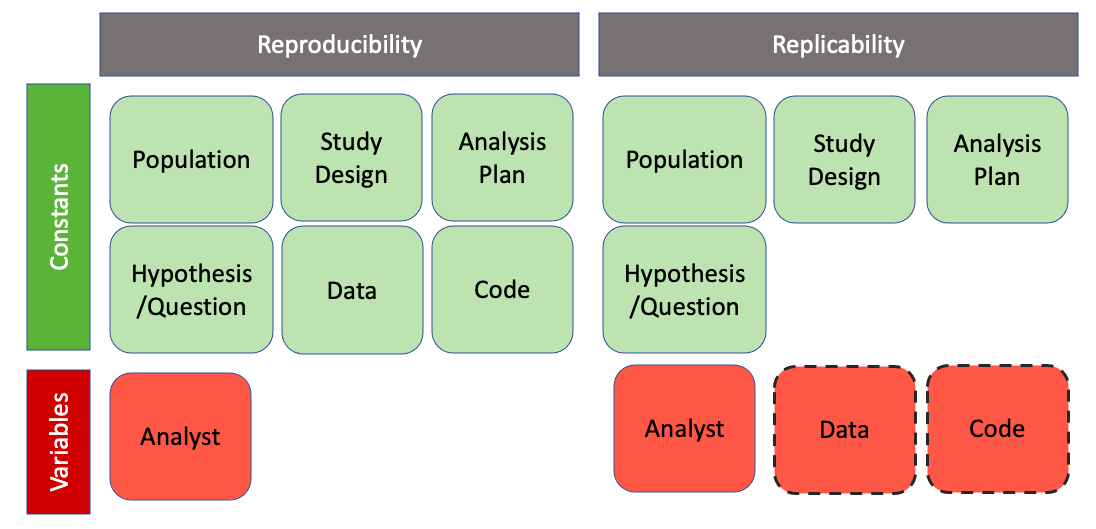
\includegraphics[width=1\linewidth]{figure/versus}

Reproducibility and replicability are both necessary to the advancement
of scientific research, but they vary significantly in terms of their
difficulty to achieve. Reproducibility, in theory, is somewhat simple to
attain in data analyses--because code is inherently non-random
(excepting applications involving random number generation) and data
remain consistent, variability is highly restricted. The achievement of
replicability, on the other hand, is a much more complex challenge,
involving significantly more variablility and requiring high quality
data, effective study design, and incredibly robust hypotheses.

\section{The Reproducibility Crisis}\label{the-reproducibility-crisis}

Despite the relative simplicity of achieving reproducibility, a
significant proportion of the work produced in the scientific community
fails to meet reproducibility standards. 52\% of respondents in a 2016
Nature survey believed that science was going through a ``crisis'' of
reproducibility. Additionally, the vast majority of researchers across
all fields studied reported having been unable to reproduce another
researcher's results, while approximately half reported having been
unable to reproduce their own.
\url{https://www.nature.com/news/1-500-scientists-lift-the-lid-on-reproducibility-1.19970}
Other studies paint an even bleaker picture: a 2015 study found that
over 50\% of studies psychology failed reproducibility tests and
research from 2012 found that figure closer to 90\% in the field of
cancer biology.
(\url{https://www.nature.com/news/over-half-of-psychology-studies-fail-reproducibility-test-1.18248},
\url{https://www.nature.com/articles/483531a})

In the past several years, this ``crisis'' of reproducibility has risen
toward the forefront of scientific discussion. Without reproducibility,
the scientific community cannot properly verify study results.This makes
it difficult to identify which information should be believed and which
should not and increases the likelihood that studies sharing misleading
information will be dispersed. The rise of data-driven technologies,
alongside our newly founded ability to instantly share knowledge
worldwide, has made reproducibility increasingly critical to the
advancement of scientific understanding, necessitating the development
of solutions for addressing the issue.

Academics have recognized this, and publications on the topic appear to
have increased siginficantly in the last several years (Eisner (2018);
Fidler \& Wilcox (2018); Gosselin (2020); McArthur (2019); Wallach,
Boyack, \& Ioannidis (2018)).

\section{The Components of Reproducible
Research}\label{the-components-of-reproducible-research}

In order to address the lack of reproducibility in scientific research,
it is important to first consider the question: Which components are
necessary to declare research reproducibile?

Publications attempting to answer this can be found in all areas of
scientific research. However, as Goodman et al. (2016) argue, the
language and conceptual framework used to describe research
reproducibility varies significantly across the sciences, and there are
no clear standards on reproducibility agreed upon by the scientific
community as a whole.

At a minimum, according to Goodman et al. (2016), documenting
reproducibility requires the sharing of data (raw or processed),
relevant metadata, code, and related software. However, according to
other authors, the full achievement of reproducibility may require
additional components.

Kitzes, Turek, \& Deniz (2017) present a collection of case studies on
reproducibility practices from across the data-intensive sciences,
illustrating a variety of recommendations and techniques for achieving
reproducibility. Although their work does not come to a consensus on the
exact standards of reproducibility that should be followed, several
common trends and principles emerge from their case studies that extend
beyond the minimum recommendations of Goodman et al. (2016):
\begin{enumerate}
\def\labelenumi{\arabic{enumi})}
\tightlist
\item
  use clear separation, labeling, and documentation in provided code,
\item
  automate processes when possible, and
\item
  design the data analysis workflow as a sequence of small steps glued
  together, with outputs from one step serving as inputs into the next.
  This is a common suggestion within the computing community,
  originating as part of the Unix philosophy (Gancarz (2003)).
\end{enumerate}
Cooper et al. (2017) focus on data analysis completed in \texttt{R} and
identify a similar list of important reproducibility components,
reinforcing the need for clearly labeled, well-documented, and
well-separated files. In addition, they recommend publishing a list of
software dependencies and using version control to track project changes
over time.

Broman (2019) reiterates the need for clear naming and file separation
while sharing several additional suggestions: keep the project contained
in one directory, use relative paths when accessing the file system, and
include a \texttt{README} file describing the project.

The reproducibility recommendations from R OpenSci, a non-profit
initiative founded in 2011 to make scientific data retrieval
reproducible, share similar principles to those discussed previously.
They focus on a need for a well-developed file system, with no
extraneous files and clear labeling. They also reiterate the need to
note dependencies and use automation when possible, while making clear a
suggestion not present in the previously-discussed literature: the need
to use seeds, which allow for the saving and restoring of the random
number generator state, when running code involving randomness (Martinez
et al. (2018)).

Although these recommendations differ from one another, when considered
in combination they provide a well-rounded picture of the components
important to research reproducibility across the scientific community:
\begin{enumerate}
\def\labelenumi{\arabic{enumi}.}
\tightlist
\item
  The basic project components are made accessible:
\end{enumerate}
\begin{itemize}
\tightlist
\item
  Data (raw and/or processed)
\item
  Metadata
\item
  Code
\item
  Related Software
\end{itemize}
\begin{enumerate}
\def\labelenumi{\arabic{enumi}.}
\setcounter{enumi}{1}
\tightlist
\item
  The file structure of project is well-organized:
\end{enumerate}
\begin{itemize}
\tightlist
\item
  Separate folders for different file types.
\item
  No extraneous files.
\item
  Minimal clutter.
\end{itemize}
\begin{enumerate}
\def\labelenumi{\arabic{enumi}.}
\setcounter{enumi}{2}
\tightlist
\item
  The project is documented well:
\end{enumerate}
\begin{itemize}
\tightlist
\item
  Files are clearly named, preferably in a way where the order in which
  they should be run is clear.
\item
  A README is present.
\item
  Software dependencies are noted.
\end{itemize}
\begin{enumerate}
\def\labelenumi{\arabic{enumi}.}
\setcounter{enumi}{3}
\tightlist
\item
  File paths used in code are not system- or user-dependent:
\end{enumerate}
\begin{itemize}
\tightlist
\item
  No absolute paths.
\item
  No paths leading to locations outside of a project's directory.
\item
  Only relative paths, pointing to locations within a project's
  directory, are permitted.
\end{itemize}
\begin{enumerate}
\def\labelenumi{\arabic{enumi}.}
\setcounter{enumi}{4}
\tightlist
\item
  Randomness is accounted for:
\end{enumerate}
\begin{itemize}
\tightlist
\item
  If randomness is used in code, a seed must also be set.
\end{itemize}
\begin{enumerate}
\def\labelenumi{\arabic{enumi}.}
\setcounter{enumi}{5}
\tightlist
\item
  Readable, styled code:
\end{enumerate}
\begin{itemize}
\tightlist
\item
  Though not mentioned in the sources described previously, it is also
  important that code be written in a coherent style. This is because
  code that conforms to a style guide or is written in a consistent
  dialect is easier to read, simplifying the process of following a
  researcher's work from beginning to end (Hermans \& Aldewereld
  (2017)).
\end{itemize}
\section{Current Attempts to Address Reproducibility in Scientific
Publishing}\label{current-attempts-to-address-reproducibility-in-scientific-publishing}

\subsection{Case Studies in Journal Reproducibility Policy Across The
Sciences}\label{case-studies-in-journal-reproducibility-policy-across-the-sciences}

In an attempt to increase reproducibility in the sciences, leaders from
academic journals around the world have taken steps to create new
standards and requirements for submitted articles. However, these
standards are highly inconsistent, varying significantly both across and
within disciplines.

The journal whose requirements appear to align most closely with those
components defined previously in Section 3 is the \emph{American Journal
of Political Science} (AJPS). In 2012, the AJPS became the first
political science journal to require authors to make their data openly
accessible online, and the publication has instituted stricter
requirements since. AJPS now requires that authors submit the following
alongside their papers:
\begin{itemize}
\tightlist
\item
  The dataset analyzed in the paper and information about its source. If
  the dataset has been processed, instructions for manipulating the raw
  data to achieve the final data must also be shared.
\item
  Detailed, clear code necessary for reproducing all of the tables and
  figures in the paper.
\item
  Documentation, including a README and codebook.
\item
  Information about the software used to conduct the analysis, including
  the specific versions and packages used.
\end{itemize}
\textbf{ADD SOURCE:}
\url{https://ajps.org/wp-content/uploads/2018/05/ajps_replication-guidelines-2-1.pdf}

These standards are quite thorough and contain mandates for the
inclusion of the vast majority of components necessary for complete
reproducibility.

Most journals, however, do not come close to meeting such high standards
in their reproducibility statements. We will consider examples from
several fields:

In the biomedical sciences, a group of editors reproesenting over 30
major journals met in 2014 to address reproducibility in their field,
coming to a consensus on a set of principles they wanted to uphold.
Listed below are those relating specifically to the use of data and
statistical methods:
\begin{enumerate}
\def\labelenumi{\arabic{enumi})}
\item
  Journals in the biomedical sciences should have a mechanism to check
  the statistical accuracy of submissions.
\item
  Journals should have no (or generous) limit on methods section length.
\item
  Journals should use a checklist to ensure the reporting of key
  information, including:
\end{enumerate}
\begin{itemize}
\tightlist
\item
  The article meets nomenclature/reporting standards of the biomedical
  field.
\item
  Investigators report how often each experiment was performed and
  whether results were substantiated by repetition under a range of
  conditions.
\item
  Statistics must be fully reported in the paper (including test used,
  value of N, definition of center, dispersion and precision measures).
\item
  Authors must state whether samples were randomized and how.
\item
  Authors must state whether the experiment was blinded.
\item
  Authors must clearly state the criteria used for exclusion of any data
  or subjects and must include all results, even those that do not
  support the main findings.
\end{itemize}
\begin{enumerate}
\def\labelenumi{\arabic{enumi})}
\setcounter{enumi}{3}
\item
  All datasets used in analysis must be made available on request and
  should be hosted on public repositories when possible. If not
  possible, data values should be presented in the paper or
  supplementary information.
\item
  Software sharing should be encouraged. At the minimum, authors should
  provide a statement describing if software is available and how to
  obtain it.
\end{enumerate}
\textbf{ADD SOURCE:}
\url{https://www.nature.com/news/journals-unite-for-reproducibility-1.16259}

Even though these principles seem well-developed on the surface, they
fail to meet even the basic requirements defined by Goodman et al.
(2016) previously. Several of the principles are purely recommendations;
there is no \emph{requirement} that code be shared, nor metadata, and
software requirements are quite loose, requiring no information about
dependencies or software version.

We see a similar issue even in journals designed specifically for the
purpose of improving scientific reproducibility. \emph{Experimental
Results}, a publication created by Cambridge University Press to address
some of the reproducibility and open access issues in academia, also
falls short of meeting high standards. The journal, which showcases
articles from a variety of scientific decisions disciplines, states in
their transparency and openness policy:
\begin{quote}
Whenever possible authors should make evidence and resources that
underpin published findings, such as data, code, and other materials,
available to readers without undue barriers to access.
\end{quote}
The inclusion of code and data are only recommended and no definition of
what ``other materials'' may mean is provided. No components of
reproducibility extending beyond those required at a minimum are even
considered.

\textbf{ADD SOURCE:}
\url{https://www.cambridge.org/core/journals/experimental-results/information/transparency-and-openness-policy}

The \emph{American Economic Review}, the first of the top economics
journals to require the inclusion of data alongside publications, has
stronger guidelines than several of those mentioned previously, though
not as strong as the \emph{American Journal of Political Science}. Their
Data and Code Availability Policy states the following:
\begin{quote}
It is the policy of the American Economic Association to publish papers
only if the data and code used in the analysis are clearly and precisely
documented, and access to the data and code is clearly and precisely
documented and is non-exclusive to the authors.
\end{quote}
SOURCE: \url{https://www.aeaweb.org/journals/policies/data-code}

These requirements are quite strict, prohibiting exceptions for papers
using data or code not available to the public in the way that many
other journals claiming to promote reproducibility do.

\subsection{Case Studies In The Statistical And Data
Sciences}\label{case-studies-in-the-statistical-and-data-sciences}

In the field of statistical and data sciences, the majority of highly
ranked journals contain statements on reproducibility. Some of these are
quite robust, surpassing the requirements of many of the other journals
discussed previously, while others are lacking.

The \emph{Journal of the American Statistical Association} stands out as
having relatively robust requirements. The publication's guideliens
require that data be made publicly available at the time of publication
except for reasons of security or confidentiality. It is strongly
recommended that code be deposited in open repositories. If data is used
in a process form, the provided code should include the necessary
cleaning/preparation steps. Data must be in an easily understood form
and a data dictionary should be included. Code should also be in a form
that can be used and understood by others, including consistent and
readable syntax and comments. Workflows involving more than one script
should also contain a master script, Makefile, or other mechanism that
makes it clear what each component does, in what order to run them, and
what the inputs and outputs to each area. \textbf{Source here:}
\url{https://jasa-acs.github.io/repro-guide/pages/author-guidelines}

The \emph{Journal of Statistical Software} also has strong guidelines,
though less thorough. Authors must provide \emph{commented} source code
for their software; all figures, tables, and output must be exactly
reproducible on at least one platform, and random number generation must
be controlled; and replication materials (typically in the form of a
script) must be provided. \textbf{Source here:}
\url{https://www.jstatsoft.org/pages/view/authors\#review-process}.

The expectations of the \emph{Journal of Computational and Graphical
Statistics} are notably weaker, requiring only that authors ``submit
code and datasets as online supplements to the manuscript,'' with
exceptions for security or confidentiality, but providing no further
detail. \textbf{Source:}
\url{https://www.tandfonline.com/action/authorSubmission?show=instructions\&journalCode=ucgs20}.
The \emph{R Journal} has the same requirements, but with no exceptions
on the data provision policy, stating that authors should ``not use such
datasets as examples.'' \textbf{Source}
\url{https://journal.r-project.org/share/author-guide.pdf}

Perhaps the weakest reproducibility policies come from \emph{The
American Statistician} and the \emph{Annals of Statistics}. The former
appears to have no requirements, stating only that it ``strongly
encourages authors to submit datasets, code, other programs, and/or
appendices that are directly relevant to their submitted articles,''
while the latter appears to have no statement on reproducibility at all.
\textbf{Sources:}
\url{https://www.tandfonline.com/action/authorSubmission?show=instructions\&journalCode=utas20},
\url{https://imstat.org/journals-and-publications/annals-of-statistics/annals-of-statistics-manuscript-submission/}.
\begin{Shaded}
\begin{Highlighting}[]
\NormalTok{knitr}\OperatorTok{::}\KeywordTok{include_graphics}\NormalTok{(}\StringTok{"figure/stats-journals.png"}\NormalTok{)}
\end{Highlighting}
\end{Shaded}
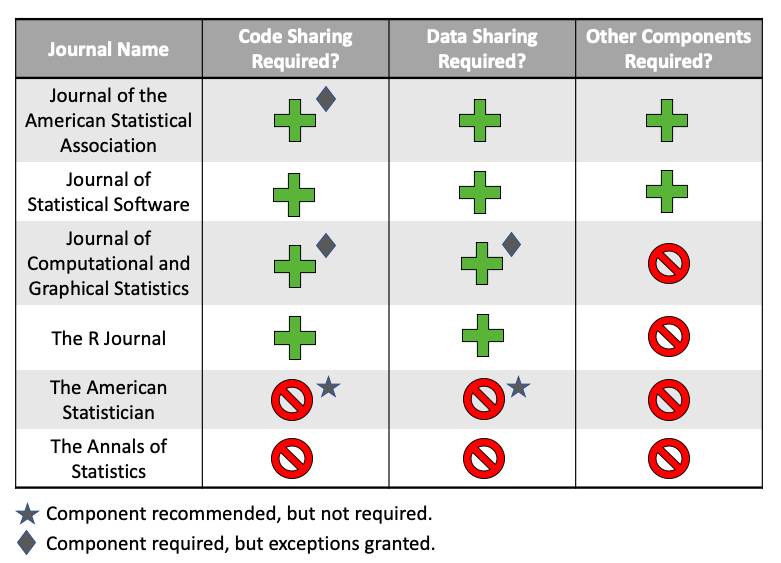
\includegraphics[width=1\linewidth]{figure/stats-journals}

\subsection{The Big Picture: Reproducibility Across
Academia}\label{the-big-picture-reproducibility-across-academia}

While previously we have focused on several case studies, it is
important to also consider the wider view of the state of
reproducibility policy across scientific journals. Are the examples
considered previously relatively standard, or are their policies either
stronger or weaker than the average policy in academia?

Academics at the Center for Open Science (COS) attempted to create a
metric, called the TOP Factor, to help answer this. The TOP Factor
reports the steps that a journal is taking to implement open science
practices. Publications receive a score from 0 to 3 based on how well
they achieve different aspects of open science:
\begin{itemize}
\tightlist
\item
  Data citation
\item
  Data transparency
\item
  Analytical code transparency
\item
  Materials transparency
\item
  Reporting guidelines
\item
  Study preregistration
\item
  Replication
\item
  Publication Bias
\end{itemize}
A journal's final score is the sum of the individual scores in each of
the categories. The full rubric for how the scores are calculated can be
found at the following site: \url{https://osf.io/t2yu5/}.

When looking at the overall distribution of TOP Factor scores, we see a
relatively grim picture: Around 50\% of journals score as low as 0-5
overall, while only just over 5\% score more than 15, just half of the
maximum possible score. Over 40 journals failed to score a single point.
\textbf{Source}:
\url{https://www.natureindex.com/news-blog/top-factor-rates-journals-on-transparency-openness}

Although it is clear that some journals have relatively strong
reproducibility and openness policies, that is clearly not the norm. And
many that do appear to have policies lacking in robustness, including
exceptions for data privacy and security concerns or phrasing guidelines
as recommendations rather than reqquirements. The field of data science
stands out among the rest, with the majority of top journals having
relatively robust policies.

\subsection{Assessing the Success of Academic Reproducibility
Policies}\label{assessing-the-success-of-academic-reproducibility-policies}

We have seen that, although not necessarily the standard, many journals
across the sciences have enacted reproducibility policies. The simple
implementation of a policy, however, does not ensure that its goals will
be achieved. Reproducibility can only be addressed when both authors
\emph{and} journal reviewers actively implement publishing standards in
practice. Without participation and dedication from all involved,
reproducibility guidelines serve more as a theoretical goal than a
practical achievement.

It is important to ask, then, whether academic reproducibility standards
\emph{actually} result in a greater number of reproducible publications.

Let us consider the case of the journal \emph{Science}. \emph{Science}
instituted a reproducibility policy in 2011 and has maintained it ever
since. In its original form, their policy stated the following:
\begin{quote}
All data necessary to understand, assess, and extend the conclusions of
the manuscript must be available to any reader of Science. All computer
codes involved in the creation or analysis of data must also be
available to any reader of Science. After publication, all reasonable
requests for data and materials must be fulfilled. Any restrictions on
the availability of data, codes, or materials\ldots{}must be disclosed
to the editors upon submission\ldots{}
\end{quote}
This policy is similar to many of the others considered previously,
requiring the publishing of code and data with exceptions permitted when
necessary.

Researchers Victoria Stodden, Jennifer Seiler, and Zhaokun Ma
(\url{https://www.pnas.org/content/115/11/2584}) tested the efficacy of
this policy in practice, emailing corresponding authors of 204 articles
published in the year after \emph{Science} first implmented its policy
to request the data and code associated with their articles. The
researchers only received (at least some of) the requested material from
36\% of authors. This low rates were due to several factors:
\begin{itemize}
\tightlist
\item
  26\% of authors did not respond to email contact.
\item
  11\% of authors were unwilling to provide the data or code without
  further information regarding the researchers' intentions.
\item
  11\% asked the researchers to contact someone else and that person did
  not respond.
\item
  7\% refused to share data and/or code.
\item
  3\% directed the researchers back to their paper's supplmental
  information section.
\item
  3\% of authors made a promise to follow up and then did not follow
  through.
\item
  3\% of emails bounced.
\item
  2\% gave reasons why they could not share for ethical reasons, size
  limitations, or some other reason.
\end{itemize}
Of the 56 papers they deemed likely reproducible, the authors randomly
selected 22 and were able to replicate the results for all but 1, which
failed due to its reliance on software that was no longer available.

A similar study was done on the journal \emph{Cognition}, where
researchers compared the reproducibility of published work both before
and after the journal instituted an open data policy, which required
that authors make relevant research data publicly available prior to
publication of an article.

The researchers found a considerable increase in the proportion of data
available statements (in constrast to `data not available' statements,
which could be present due to privacy or security concerns) since the
implementation of the policy. Pre-open data policy, only 25\% of
articles had data available, while that number was a much higher 78\%
after the policy was put in place.

While the institution of an open data policy appears to have been
associated with a significant increase in the percentage of studies with
data available, further research indicates that the policy was perhaps
not as effective as intended. Many of the datasets were usable in
theory, but not in practice. Only 62\% of the articles with data
available statements had truly reusable datasets--in this case, meaning
that the data were accessible, complete, and understandable. Though this
is an increase from the pre-policy period, which saw 49\% of articles
with data availability statements as reusable in practice, it is still
far from ideal.

Combining these two data points indicates that \emph{less than half} of
articles published after the open data policy was instituted actually
contained truly usable data.

\textbf{Source}
\url{https://royalsocietypublishing.org/doi/full/10.1098/rsos.180448}

In this small sample of cases, we see that purely having a
reproducibility statement does not necessarily mean that all, or even a
majority, of published work will truly be reproducible.

\section{Limitations on Achieving
Reproducibility}\label{limitations-on-achieving-reproducibility}

There are several reasons for this apparent divide between journal
reproducibility standards and the true proportion of submitted articles
that are truly reproducible. Some of these are challenges faced by the
article authors, while others are faced by the journal editors.

\subsection{Challenges for Authors}\label{challenges-for-authors}

A \emph{Springer Nature} survey asked over 7,700 researchers about one
of the key characteristics of reproducibility -- open data -- and
gathered information about the reasons why authors found difficulties in
making their data available to the public.

The main challenges listed by respondents were as follows:
\begin{itemize}
\tightlist
\item
  46\% identified ``Organizing data in a presentable and useful way'' to
  be difficult.
\item
  37\% had been ``Unsure about copyright and licensing.''
\item
  33\% had problems with ``Not knowing which repository to use.''
\item
  26\% cited a ``Lack of time to deposit data.''
\item
  19\% found the ``Costs of sharing data'' to be high.
\end{itemize}
The relative frequency of these issues varied across several
characteristics, including author seniority, subject area, and
geographical location, though authors in all categories faced some
issues.

\textbf{STUDY LINK}
\url{https://figshare.com/articles/Whitepaper_Practical_challenges_for_researchers_in_data_sharing/5975011}

Given the relatively high frequency of concern over achieving
reproducibility, it follows that researchers will not make the necessary
effort to do so if journal guidelines provide a way out. Policies that
\emph{recommend} the inclusion of data or that allow exceptions to open
data for certain reasons are likely to be associated with a lower
proportion of reproducible articles than those that make open data
mandatory.

\subsection{Challenges for Journals}\label{challenges-for-journals}

In addition to the challenges faced on the part of the authors, journal
reviewers face their own difficulties in ensuring reproducibility.

In order to make sure that all submitted articles comply with
reproducibility guidelines, reviewers must go through them one by one
and reproduce all of the results by hand using the provided materials.

This is an incredibly intensive process, as we will see in the example
of the \emph{American Journal for Political Science} (AJPS), whose
reproducibility policy was discussed prevously in Chapter 1.4.1.

Acceptance of an article for publication in the AJPS is contingent on
successful reproducibility of any empirical analyses reported in the
article.

After an article is submitted, staff from a third party vendor hired by
AJPS go through the provided materials to ensure that they can be
preserved, understood, and used by others. They then run all of the
analyses in the article using the code, instructions, and data provided
by the authors and compare their results to the submitted articles.
Authors are then given an opportunity to resolve any issues that come
up. This process is repeated until reproducibility is ensured.

Although providing a significant benefit to the scientific community,
this thorough process is associated with high costs.

The verification process slows down the journal review process
significantly, adding a median 53 days to the publication workflow, as
many submitted articles require one or more rounds of resubmission (the
average number of resubmissions is 1.7). It is also quite labor
intensive, taking an average of 8 person-hours per manuscript to
reproduce the analyses and prepare the materials for public release and
adding significant monetary cost to AJPS.

\url{https://www.insidehighered.com/blogs/rethinking-research/should-journals-be-responsible-reproducibility}

Journals are often reluctant to take on such an intensive task due to
the drastically increased burden it places on reviewers and on the
publication's financial resources. This is particularly true given that
the number of submitted articles per year has been increasing over time.
( \url{https://www.ncbi.nlm.nih.gov/pmc/articles/PMC4317455/} ) Every
additional submission increases the burden of achieving reproducibility,
and with a large enough volume, the challenge can quickly become
seemingly impossible to manage reasonably.

As a result, journals often encourage reviewers to consider authors'
compliance with data sharing policies, but do not formally require that
they ensure it as a criterion for acceptance.
\url{https://link.springer.com/chapter/10.1007/164_2019_290}

\url{http://emiguel.econ.berkeley.edu/assets/miguel_research/78/jel.20171350.pdf}

\section{Reproducibility Education}\label{reproducibility-education}

\chapter{Addressing the Challenges of
Reproducibility}\label{my-solution}

{[}

The relative simplicity of the reproducibility challenge makes it an
ideal candidate for solution-building. Although significant progress on
addressing reproducibility on a widespread scale is a long-term
challenge, impactful forward progress--if on a smaller scale--can be
achieved in the short-term.

My research has focused on doing just this, providing tools to assist
with achieving reproducibility in one segment of the scientific
community: RStudio users.

{]} --- DO WE NEED THIS?

\section{Review Of Previous Work}\label{review-of-previous-work}

\subsection{R Packages and Other
Software}\label{r-packages-and-other-software}

Much of this work is highly generalized, written to be applicable to
users working with a variety of statistical software programs. Because
all statistical software programs operate differently, these
recommendations are inherently vague and difficult to implement,
particularly to new analysts who are relatively unfamiliar with their
software. Focused attempts to address reproducibility in specific
certain software programs are more likely to be successful. We focus on
\texttt{R}, due to its open-source nature, accessibility, and popularity
as a tool for statistical analysis.

A small body of \texttt{R} packages focuses on research reproducibility.
\texttt{rrtools} (Marwick (2019)) addresses some of the issues discussed
in Marwick, Boettiger, \& Mullen (2018) by creating a basic \texttt{R}
package structure for a data analysis project and implementing a basic
\texttt{testthat::check} functionality. The \texttt{orderly} (FitzJohn
et al. (2020)) package also focuses on file structure, requiring the
user to declare a desired project structure (typically a step-by-step
structure, where outputs from one step are inputs into the next) at the
beginning and then creating the files necessary to achieve that
structure. \texttt{workflowr}'s (Blischak, Carbonetto, \& Stephens
(2019)) functionality is based around version control and making code
easily available online. It works to generate a website containing
time-stamped, versioned, and documented results. \texttt{checkers}
(Ross, DeCicco, \& Randhawa (2018)) allows you to create custom checks
that examine different aspects of reproducibility. \texttt{packrat}
(Ushey, McPherson, Cheng, Atkins, \& Allaire (2018)) is focused on
dependencies, creating a packaged folder containing a project as well as
all of its dependencies so that projects dependent on lesser-used
packages can be easily shared across computers. \texttt{drake} (OpenSci
(2020)) analyzes workflows, skips steps where results are up to date,
and provides evidence that results match the underlying code and data.
Lastly, the \texttt{reproducible} (McIntire \& Chubaty (2020)) package
focuses on the concept of caching: saving information so that projects
can be run faster each time they are re-completed from the start.

Many of these packages are narrow, with each effectively addressing a
small component of reproducibility: file structure, modularization of
code, version control, etc. These packages often succeed in their area
of focus, but at the cost of accessibility to a wider audience. Their
functions are often quite complex to use, and many steps must be
completed to achieve the required reproducibility goal. This cumbersome
nature means that most reproducibility packages currently available are
not easily accessible to users near the beginning of their \texttt{R}
journey, nor particularly useful to those looking for quick and easy
reproducibility checks. A more effective way of realizing widespread
reproducibility is to make the process for doing so simple enough that
it takes little to no conscious effort to implement. You want users to
``fall into a hole'' (we paraphrase Hadley Wickham) of good practice.

\texttt{Continuous\ integration} tools provide more general approaches
to automated checking, which can enhance reproducibility with minimal
code. For example, \texttt{wercker}---a command line tool that leverages
Docker---enables users to test whether their projects will successfully
compile when run on a variety of operating systems without access to the
user's local hard drive (Oracle Corporation (2019)).
\texttt{GitHub\ Actions} is integrated into GitHub and can be configured
to do similar checks on projects hosted in repositories.
\texttt{Travis\ CI} and \texttt{Circle\ CI} are popular continuous
integration tools that can also be used to check \texttt{R} code.

However, while these tools can be useful, they are generalized so as to
be useful to the widest audience. As a result, their checks are not
designed to be \texttt{R}-specific, which makes them sub-optimal for
users looking to address reproducibility issues involving features
specific to the \texttt{R} programming language, such as package
installation and seed setting.

\section{Identifying Gaps In Existing
Solutions}\label{identifying-gaps-in-existing-solutions}

\section{\texorpdfstring{My Contribution: \texttt{fertile}, An R Package
Creating Optimal Conditions For
Reproducibility}{My Contribution: fertile, An R Package Creating Optimal Conditions For Reproducibility}}\label{my-contribution-fertile-an-r-package-creating-optimal-conditions-for-reproducibility}

\subsection{Package Overview}\label{package-overview}

\texttt{fertile} attempts to address these gaps in existing software by
providing a simple, easy-to-learn reproducibility package that, rather
than focusing intensely on a specific area, provides some information
about a wide variety of aspects influencing reproducibility.
\texttt{fertile} is flexible, offering benefits to users at any stage in
the data analysis workflow, and provides \texttt{R}-specific features,
which address certain aspects of reproducibility that can be missed by
external project development software.

\texttt{fertile} is designed to be used on data analyses organized as
\texttt{R} Projects (i.e.~directories containing an \texttt{.Rproj}
file). Once an \texttt{R} Project is created, \texttt{fertile} provides
benefits throughout the data analysis process, both during development
as well as after the fact. \texttt{fertile} achieves this by operating
in two modes: proactively (to prevent reproducibility mistakes from
happening in the first place), and retroactively (analyzing code that
has already been written for potential problems).

Much of the available literature focuses on file structure,
organization, and naming, and \texttt{fertile}'s features are consistent
with this. Marwick et al. (2018) provide the framework for file
structure that \texttt{fertile} is based on: a structure similar to that
of an \texttt{R} package (R-Core-Team (2020), Wickham (2015)), with an
\texttt{R} folder, as well as \texttt{data}, \texttt{data-raw},
\texttt{inst}, and \texttt{vignettes}.

\subsection{Proactive Use}\label{proactive-use}

Proactively, the package identifies potential mistakes as they are made
by the user and outputs an informative message as well as a recommended
solution. For example, \texttt{fertile} catches when a user passes a
potentially problematic file path---such as an absolute path, or a path
that points to a location outside of the project directory---to a
variety of common input/output functions operating on many different
file types.
\begin{Shaded}
\begin{Highlighting}[]
\KeywordTok{library}\NormalTok{(fertile)}
\KeywordTok{file.exists}\NormalTok{(}\StringTok{"~/Desktop/my_data.csv"}\NormalTok{)}
\end{Highlighting}
\end{Shaded}
\begin{verbatim}
[1] TRUE
\end{verbatim}
\begin{Shaded}
\begin{Highlighting}[]
\KeywordTok{read.csv}\NormalTok{(}\StringTok{"~/Desktop/my_data.csv"}\NormalTok{)}
\end{Highlighting}
\end{Shaded}
\begin{verbatim}
Error: Detected absolute paths
\end{verbatim}
\begin{Shaded}
\begin{Highlighting}[]
\KeywordTok{read.csv}\NormalTok{(}\StringTok{"../../../Desktop/my_data.csv"}\NormalTok{)}
\end{Highlighting}
\end{Shaded}
\begin{verbatim}
Error: Detected paths that lead outside the project directory
\end{verbatim}
\texttt{fertile} is even more aggressive with functions (like
\texttt{setwd()}) that are almost certain to break reproducibility,
causing them to throw errors that prevent their execution and providing
recommendations for better alternatives.
\begin{Shaded}
\begin{Highlighting}[]
\KeywordTok{setwd}\NormalTok{(}\StringTok{"~/Desktop"}\NormalTok{)}
\end{Highlighting}
\end{Shaded}
\begin{verbatim}
Error: setwd() is likely to break reproducibility. Use here::here() instead.
\end{verbatim}
These proactive warning features are activated immediately after
attaching the \texttt{fertile} package and require no additional effort
by the user.

\subsection{Retroactive Use}\label{retroactive-use}

Retroactively, \texttt{fertile} analyzes potential obstacles to
reproducibility in an RStudio Project (i.e., a directory that contains
an \texttt{.Rproj} file). The package considers several different
aspects of the project which may influence reproducibility, including
the directory structure, file paths, and whether randomness is used
thoughtfully.

The end products of these analyses are reproducibility reports
summarizing a project's adherence to reproducibility standards and
recommending remedies for where the project falls short. For example,
\texttt{fertile} might identify the use of randomness in code and
recommend setting a seed if one is not present.

Users can access the majority of \texttt{fertile}'s retroactive features
through two primary functions, \texttt{proj\_check()} and
\texttt{proj\_analyze()}.

The \texttt{proj\_check()} function runs fifteen different
reproducibility tests, noting which ones passed, which ones failed, the
reason for failure, a recommended solution, and a guide to where to look
for help. These tests include: looking for a clear build chain, checking
to make sure the root level of the project is clear of clutter,
confirming that there are no files present that are not being directly
used by or created by the code, and looking for uses of randomness that
do not have a call to \texttt{set.seed()} present. A full list is
provided below:
\begin{Shaded}
\begin{Highlighting}[]
\KeywordTok{list_checks}\NormalTok{()}
\end{Highlighting}
\end{Shaded}
\begin{verbatim}
-- The available checks in `fertile` are as follows: ---------------------------------- fertile 0.0.0.9027 --
\end{verbatim}
\begin{verbatim}
 [1] "has_tidy_media"          "has_tidy_images"        
 [3] "has_tidy_code"           "has_tidy_raw_data"      
 [5] "has_tidy_data"           "has_tidy_scripts"       
 [7] "has_readme"              "has_no_lint"            
 [9] "has_proj_root"           "has_no_nested_proj_root"
[11] "has_only_used_files"     "has_clear_build_chain"  
[13] "has_no_absolute_paths"   "has_only_portable_paths"
[15] "has_no_randomness"      
\end{verbatim}
Subsets of the fifteen tests can be invoked using the
\texttt{tidyselect} helper functions (Henry \& Wickham (2020)) in
combination with the more limited \texttt{proj\_check\_some()} function.
\begin{Shaded}
\begin{Highlighting}[]
\NormalTok{proj_dir <-}\StringTok{ "project_miceps"}
\end{Highlighting}
\end{Shaded}
\begin{Shaded}
\begin{Highlighting}[]
\KeywordTok{proj_check_some}\NormalTok{(proj_dir, }\KeywordTok{contains}\NormalTok{(}\StringTok{"paths"}\NormalTok{))}
\end{Highlighting}
\end{Shaded}
\begin{verbatim}
-- Compiling... ----------------------------------------------------------------------- fertile 0.0.0.9027 --
\end{verbatim}
\begin{verbatim}
-- Rendering R scripts... ------------------------------------------------------------- fertile 0.0.0.9027 --
\end{verbatim}
\begin{verbatim}
-- Running reproducibility checks ----------------------------------------------------- fertile 0.0.0.9027 --
\end{verbatim}
\begin{verbatim}
v Checking for no absolute paths
\end{verbatim}
\begin{verbatim}
v Checking for only portable paths
\end{verbatim}
\begin{verbatim}
-- Summary of fertile checks ---------------------------------------------------------- fertile 0.0.0.9027 --
\end{verbatim}
\begin{verbatim}
v Reproducibility checks passed: 2
\end{verbatim}
Each test can also be run individually by calling the function matching
its check name.

The \texttt{proj\_analyze()} function creates a report documenting the
structure of a data analysis project. This report contains information
about all packages referenced in code, the files present in the
directory and their types, suggestions for moving files to create a more
organized structure, and a list of reproducibility-breaking file paths
used in code.
\begin{Shaded}
\begin{Highlighting}[]
\KeywordTok{proj_analyze}\NormalTok{(proj_dir)}
\end{Highlighting}
\end{Shaded}
\begin{verbatim}
-- Analysis of reproducibility for project_miceps ------------------------------------- fertile 0.0.0.9027 --
\end{verbatim}
\begin{verbatim}
--   Packages referenced in source code ----------------------------------------------- fertile 0.0.0.9027 --
\end{verbatim}
\begin{verbatim}
# A tibble: 9 x 3
  package       N used_in                    
  <chr>     <int> <chr>                      
1 broom         1 project_miceps/analysis.Rmd
2 dplyr         1 project_miceps/analysis.Rmd
3 ggplot2       1 project_miceps/analysis.Rmd
4 purrr         1 project_miceps/analysis.Rmd
5 readr         1 project_miceps/analysis.Rmd
6 rmarkdown     1 project_miceps/analysis.Rmd
7 skimr         1 project_miceps/analysis.Rmd
8 stargazer     1 project_miceps/analysis.Rmd
9 tidyr         1 project_miceps/analysis.Rmd
\end{verbatim}
\begin{verbatim}
--   Files present in directory ------------------------------------------------------- fertile 0.0.0.9027 --
\end{verbatim}
\begin{verbatim}
                     file   ext    size
1 Estrogen_Receptors.docx  docx  10.97K
2      citrate_v_time.png   png 187.83K
3     proteins_v_time.png   png 376.94K
4   Blot_data_updated.csv   csv  14.43K
5      CS_data_redone.csv   csv   7.39K
6                mice.csv   csv  14.33K
7               README.md    md      39
8            miceps.Rproj Rproj     204
9            analysis.Rmd   Rmd   4.94K
                                                                     mime
1 application/vnd.openxmlformats-officedocument.wordprocessingml.document
2                                                               image/png
3                                                               image/png
4                                                                text/csv
5                                                                text/csv
6                                                                text/csv
7                                                           text/markdown
8                                                            text/rstudio
9                                                         text/x-markdown
\end{verbatim}
\begin{verbatim}
--   Suggestions for moving files ----------------------------------------------------- fertile 0.0.0.9027 --
\end{verbatim}
\begin{verbatim}
                 path_rel    dir_rel
1   Blot_data_updated.csv   data-raw
2      CS_data_redone.csv   data-raw
3 Estrogen_Receptors.docx inst/other
4            analysis.Rmd  vignettes
5      citrate_v_time.png inst/image
6                mice.csv   data-raw
7     proteins_v_time.png inst/image
                                                                                               cmd
1     file_move('project_miceps/Blot_data_updated.csv', fs::dir_create('project_miceps/data-raw'))
2        file_move('project_miceps/CS_data_redone.csv', fs::dir_create('project_miceps/data-raw'))
3 file_move('project_miceps/Estrogen_Receptors.docx', fs::dir_create('project_miceps/inst/other'))
4             file_move('project_miceps/analysis.Rmd', fs::dir_create('project_miceps/vignettes'))
5      file_move('project_miceps/citrate_v_time.png', fs::dir_create('project_miceps/inst/image'))
6                  file_move('project_miceps/mice.csv', fs::dir_create('project_miceps/data-raw'))
7     file_move('project_miceps/proteins_v_time.png', fs::dir_create('project_miceps/inst/image'))
\end{verbatim}
\begin{verbatim}
--   Problematic paths logged --------------------------------------------------------- fertile 0.0.0.9027 --
\end{verbatim}
\begin{verbatim}
NULL
\end{verbatim}
\subsection{Logging}\label{logging}

\texttt{fertile} also contains logging functionality, which records
commands run in the console that have the potential to affect
reproducibility, enabling users to look at their past history at any
time. The package focuses mostly on package loading and file opening,
noting which function was used, the path or package it referenced, and
the timestamp at which that event happened. Users can access the log
recording their commands at any time via the \texttt{log\_report()}
function:
\begin{Shaded}
\begin{Highlighting}[]
\KeywordTok{log_report}\NormalTok{()}
\end{Highlighting}
\end{Shaded}
\begin{verbatim}
# A tibble: 6 x 4
  path        path_abs                    func     timestamp          
  <chr>       <chr>                       <chr>    <dttm>             
1 package:re~ <NA>                        base::r~ 2020-09-10 17:49:08
2 package:th~ <NA>                        base::r~ 2020-09-10 17:49:08
3 package:th~ <NA>                        base::l~ 2020-09-10 17:49:08
4 package:pu~ <NA>                        base::l~ 2020-09-10 17:50:09
5 package:fo~ <NA>                        base::l~ 2020-09-10 17:50:09
6 project_mi~ /Users/audreybertin/Docume~ readr::~ 2020-09-10 17:50:09
\end{verbatim}
The log, if not managed, can grow very long over time. For users who do
not desire such functionality, \texttt{log\_clear()} provides a way to
erase the log and start over.

\subsection{Utility Functions}\label{utility-functions}

\texttt{fertile} also provides several useful utility functions that may
assist with the process of data analysis.

\subsection{File Path Management}\label{file-path-management}

The \texttt{check\_path()} function analyzes a vector of paths (or a
single path) to determine whether there are any absolute paths or paths
that lead outside the project directory.
\begin{Shaded}
\begin{Highlighting}[]
\CommentTok{# Path inside the directory}
\KeywordTok{check_path}\NormalTok{(}\StringTok{"project_miceps"}\NormalTok{)}
\end{Highlighting}
\end{Shaded}
\begin{verbatim}
# A tibble: 0 x 3
# ... with 3 variables: path <chr>, problem <chr>, solution <chr>
\end{verbatim}
\begin{Shaded}
\begin{Highlighting}[]
\CommentTok{# Absolute path (current working directory)}
\KeywordTok{check_path}\NormalTok{(}\KeywordTok{getwd}\NormalTok{())}
\end{Highlighting}
\end{Shaded}
\begin{verbatim}
Error: Detected absolute paths
\end{verbatim}
\begin{Shaded}
\begin{Highlighting}[]
\CommentTok{# Path outside the directory}
\KeywordTok{check_path}\NormalTok{(}\StringTok{"../fertile.Rmd"}\NormalTok{)}
\end{Highlighting}
\end{Shaded}
\begin{verbatim}
Error: Detected paths that lead outside the project directory
\end{verbatim}
\subsection{File Types}\label{file-types}

There are several functions that can be used to check the type of a
file:
\begin{Shaded}
\begin{Highlighting}[]
\KeywordTok{is_data_file}\NormalTok{(fs}\OperatorTok{::}\KeywordTok{path}\NormalTok{(proj_dir, }\StringTok{"mice.csv"}\NormalTok{))}
\end{Highlighting}
\end{Shaded}
\begin{verbatim}
[1] TRUE
\end{verbatim}
\begin{Shaded}
\begin{Highlighting}[]
\KeywordTok{is_image_file}\NormalTok{(fs}\OperatorTok{::}\KeywordTok{path}\NormalTok{(proj_dir, }\StringTok{"proteins_v_time.png"}\NormalTok{))}
\end{Highlighting}
\end{Shaded}
\begin{verbatim}
[1] TRUE
\end{verbatim}
\begin{Shaded}
\begin{Highlighting}[]
\KeywordTok{is_text_file}\NormalTok{(fs}\OperatorTok{::}\KeywordTok{path}\NormalTok{(proj_dir, }\StringTok{"README.md"}\NormalTok{))}
\end{Highlighting}
\end{Shaded}
\begin{verbatim}
[1] TRUE
\end{verbatim}
\begin{Shaded}
\begin{Highlighting}[]
\KeywordTok{is_r_file}\NormalTok{(fs}\OperatorTok{::}\KeywordTok{path}\NormalTok{(proj_dir, }\StringTok{"analysis.Rmd"}\NormalTok{))}
\end{Highlighting}
\end{Shaded}
\begin{verbatim}
[1] TRUE
\end{verbatim}
\subsection{Temporary Directories}\label{temporary-directories}

The \texttt{sandbox()} function allows the user to make a copy of their
project in a temporary directory. This can be useful for ensuring that
projects run properly when access to the local file system is removed.
\begin{Shaded}
\begin{Highlighting}[]
\NormalTok{proj_dir}
\end{Highlighting}
\end{Shaded}
\begin{verbatim}
[1] "project_miceps"
\end{verbatim}
\begin{Shaded}
\begin{Highlighting}[]
\NormalTok{fs}\OperatorTok{::}\KeywordTok{dir_ls}\NormalTok{(proj_dir) }\OperatorTok\StringTok{ }\KeywordTok{head}\NormalTok{(}\DecValTok{3}\NormalTok{)}
\end{Highlighting}
\end{Shaded}
\begin{verbatim}
project_miceps/Blot_data_updated.csv
project_miceps/CS_data_redone.csv
project_miceps/Estrogen_Receptors.docx
\end{verbatim}
\begin{Shaded}
\begin{Highlighting}[]
\NormalTok{temp_dir <-}\StringTok{ }\KeywordTok{sandbox}\NormalTok{(proj_dir)}
\NormalTok{temp_dir}
\end{Highlighting}
\end{Shaded}
\begin{verbatim}
/var/folders/v6/f62qz88s0sd5n3yqw9d8sb300000gn/T/RtmpHyiqPk/project_miceps
\end{verbatim}
\begin{Shaded}
\begin{Highlighting}[]
\NormalTok{fs}\OperatorTok{::}\KeywordTok{dir_ls}\NormalTok{(temp_dir) }\OperatorTok\StringTok{ }\KeywordTok{head}\NormalTok{(}\DecValTok{3}\NormalTok{)}
\end{Highlighting}
\end{Shaded}
\begin{verbatim}
/var/folders/v6/f62qz88s0sd5n3yqw9d8sb300000gn/T/RtmpHyiqPk/project_miceps/Blot_data_updated.csv
/var/folders/v6/f62qz88s0sd5n3yqw9d8sb300000gn/T/RtmpHyiqPk/project_miceps/CS_data_redone.csv
/var/folders/v6/f62qz88s0sd5n3yqw9d8sb300000gn/T/RtmpHyiqPk/project_miceps/Estrogen_Receptors.docx
\end{verbatim}
\subsection{Managing Project
Dependencies}\label{managing-project-dependencies}

One of the challenges with ensuring that work is reproducible is the
issue of dependencies. Many data analysis projects reference a variety
of \texttt{R} packages in their code. When such projects are shared with
other users who may not have the required packages downloaded, it can
cause errors that prevent the project from running properly.

The \texttt{proj\_pkg\_script()}\} function assists with this issue by
making it simple and fast to download dependencies. When run on an
\texttt{R} project directory, the function creates a \texttt{.R} script
file that contains the code needed to install all of the packages
referenced in the project, differentiating between packages located on
CRAN and those located on GitHub.
\begin{Shaded}
\begin{Highlighting}[]
\NormalTok{install_script <-}\StringTok{ }\KeywordTok{proj_pkg_script}\NormalTok{(proj_dir)}
\KeywordTok{cat}\NormalTok{(}\KeywordTok{readChar}\NormalTok{(install_script, }\FloatTok{1e5}\NormalTok{))}
\end{Highlighting}
\end{Shaded}
\begin{verbatim}
# Run this script to install the required packages for this R project.
# Packages hosted on CRAN...
install.packages(c( 'broom', 'dplyr', 'ggplot2', 'purrr', 'readr', 'rmarkdown', 'skimr', 'stargazer', 'tidyr' ))
# Packages hosted on GitHub...
\end{verbatim}
\section{\texorpdfstring{How \texttt{fertile}
Works}{How fertile Works}}\label{how-fertile-works}

Much of the functionality in \texttt{fertile} is achieved by writing
\texttt{shims} \textbf{link to wikipedia page here}. \texttt{fertile}'s
shimmed functions intercept the user's commands and perform various
logging and checking tasks before executing the desired function. Our
process is:
\begin{enumerate}
\def\labelenumi{\arabic{enumi}.}
\item
  Identify an \texttt{R} function that is likely to be involved in
  operations that may break reproducibility. Popular functions
  associated with only one package (e.g., \texttt{read\_csv()} from
  \texttt{readr}) are ideal candidates.
\item
  Create a function in \texttt{fertile} with the same name that takes
  the same arguments (and always the dots \texttt{...}).
\item
  Write this new function so that it:
\end{enumerate}
\begin{enumerate}
\def\labelenumi{\alph{enumi})}
\tightlist
\item
  captures any arguments,
\item
  logs the name of the function called,
\item
  performs any checks on these arguments, and
\item
  calls the original function with the original arguments. Except where
  warranted, the execution looks the same to the user as if they were
  calling the original function.
\end{enumerate}
Most shims are quite simple and look something like what is shown below
for \texttt{read\_csv()}.
\begin{Shaded}
\begin{Highlighting}[]
\NormalTok{fertile}\OperatorTok{::}\NormalTok{read_csv}
\end{Highlighting}
\end{Shaded}
\begin{verbatim}
function(file, ...) {
  if (interactive_log_on()) {
    log_push(file, "readr::read_csv")
    check_path_safe(file)
    readr::read_csv(file, ...)
  }
}
<bytecode: 0x7feeaf5a6db8>
<environment: namespace:fertile>
\end{verbatim}
\texttt{fertile} shims many common functions, including those that read
in a variety of data types, write data, and load packages. This works
both proactively and retroactively, as the shimmed functions written in
\texttt{fertile} are activated both when the user is coding
interactively and when a file containing code is rendered.

In order to ensure that the \texttt{fertile} versions of functions
(``shims'') always supersede (``mask'') their original namesakes when
called, \texttt{fertile} uses its own shims of the \texttt{library} and
\texttt{require} functions to manipulate the \texttt{R} \texttt{search}
path so that it is always located in the first position. In the
\texttt{fertile} version of \texttt{library()}, we detach
\texttt{fertile} from the search path, load the requested package, and
then re-attach \texttt{fertile}. This ensures that when a user executes
a command, \texttt{R} will check \texttt{fertile} for a matching
function before considering other packages. While it is possible that
this shifty behavior could lead to unintended consequences, our goal is
to catch a good deal of problems before they become problematic. Users
can easily disable \texttt{fertile} by detaching it, or not loading it
in the first place.

\section{\texorpdfstring{\texttt{fertile} in Practice: Experimental
Results From Smith College Student
Use}{fertile in Practice: Experimental Results From Smith College Student Use}}\label{fertile-in-practice-experimental-results-from-smith-college-student-use}

\texttt{fertile} is designed to: 1) be simple enough that users with
minimal \texttt{R} experience can use the package without issue, 2)
increase the reproducibility of work produced by its users, and 3)
educate its users on why their work is or is not reproducible and
provide guidance on how to address any problems.

To test \texttt{fertile}'s effectiveness, we began an initial randomized
control trial of the package on an introductory undergraduate data
science course at Smith College in Spring 2020 \textbf{ADD FOOTNOTE}
(This study was approved by Smith College IRB, Protocol \#19-032).

The experiment was structured as follows:

1.Students are given a form at the start of the semester asking whether
they consent to participate in a study on data science education. In
order to successfully consent, they must provide their system username,
collected through the command \texttt{Sys.getenv("LOGNAME")}. To
maintain privacy the results are then transformed into a hexadecimal
string via the \texttt{md5()} hashing function.
\begin{enumerate}
\def\labelenumi{\arabic{enumi}.}
\setcounter{enumi}{1}
\item
  These hexadecimal strings are then randomly assigned into equally
  sized groups, one experimental group that receives the features of
  \texttt{fertile} and one group that receives a control.
\item
  The students are then asked to download a package called
  \texttt{sds192} (the course number and prefix), which was created for
  the purpose of this trial. It leverages an \texttt{.onAttach()}
  function to scan the \texttt{R} environment and collect the username
  of the user who is loading the package and run it through the same
  hashing algorithm as used previously. It then identifies whether that
  user belongs to the experimental or the control group. Depending on
  the group they are in, they receive a different version of the
  package.
\item
  The experimental group receives the basic \texttt{sds192} package,
  which consists of some data sets and \texttt{R} Markdown templates
  necessary for completing homework assignments and projects in the
  class, but also has \texttt{fertile} installed and loaded silently in
  the background. The package's proactive features are enabled, and
  therefore users will receive warning messages when they use absolute
  or non-portable paths or attempt to change their working directory.
  The control group receives only the basic \texttt{sds192} package,
  including its data sets and \texttt{R} Markdown templates. All
  students from both groups then use their version of the package
  throughout the semester on a variety of projects.
\item
  Both groups are given a short quiz on different components of
  reproducibility that are intended to be taught by \texttt{fertile} at
  both the beginning and end of the semester. Their scores are then
  compared to see whether one group learned more than the other group or
  whether their scores were essentially equivalent. Additionally, for
  every homework assignment submitted, the professor takes note of
  whether or not the project compiles successfully.
\end{enumerate}
Based on the results, we hope to determine whether \texttt{fertile} was
successful at achieving its intended goals. A lack of notable difference
between the \emph{experimental} and \emph{control} groups in terms of
the number of code-related questions asked throughout the semester would
indicate that \texttt{fertile} achieved its goal of simplicity. A higher
average for the \emph{experimental} group in terms of the number of
homework assignments that compiled successfully would indicate that
\texttt{fertile} was successful in increasing reproducibility. A greater
increase over the semester in the reproducibility quiz scores for
students in the \emph{experimental} group compared with the
\emph{control} group would indicate that \texttt{fertile} achieved its
goal of educating users on reproducibility. Success according to these
metrics would provide evidence showing \texttt{fertile}'s benefit as
tool to help educators introduce reproducibility concepts in the
classroom.

\chapter{Incorporating Reproducibility Tools Into The Greater Data
Science Community}\label{applications}

\section{\texorpdfstring{Potential Applications of
\texttt{fertile}}{Potential Applications of fertile}}\label{potential-applications-of-fertile}

\subsection{In Journal Review}\label{in-journal-review}

\subsection{By Beginning Data
Scientists}\label{by-beginning-data-scientists}

\subsection{By Advanced Data
Scientists}\label{by-advanced-data-scientists}

\subsection{For Teaching
Reproducibily}\label{for-teaching-reproducibily}

\section{\texorpdfstring{Integration Of \texttt{fertile} And Other
Reproducibility Tools in Data Science
Education}{Integration Of fertile And Other Reproducibility Tools in Data Science Education}}\label{integration-of-fertile-and-other-reproducibility-tools-in-data-science-education}

\chapter*{Conclusion}\label{conclusion}
\addcontentsline{toc}{chapter}{Conclusion}

\texttt{fertile} is an \texttt{R} package that lowers barriers to
reproducible data analysis projects in \texttt{R}, providing a wide
array of checks and suggestions addressing many different aspects of
project reproducibility, including file organization, file path usage,
documentation, and dependencies. \texttt{fertile} is meant to be
educational, providing informative error messages that indicate why
users' mistakes are problematic and sharing recommendations on how to
fix them. The package is designed in this way so as to promote a greater
understanding of reproducibility concepts in its users, with the goal of
increasing the overall awareness and understanding of reproducibility in
the \texttt{R} community.

The package has very low barriers to entry, making it accessible to
users with various levels of background knowledge. Unlike many other
\texttt{R} packages focused on reproducibility that are currently
available, the features of \texttt{fertile} can be accessed almost
effortlessly. Many of the retroactive features can be accessed in only
two lines of code requiring minimal arguments and some of the proactive
features can be accessed with no additional effort beyond loading the
package. This, in combination with the fact that \texttt{fertile} does
not focus on one specific area of reproducibility, instead covering
(albeit in less detail) a wide variety of topics, means that
\texttt{fertile} makes it easy for data analysts of all skill levels to
quickly gain a better understanding of the reproducibility of the work.

In the moment, it often feels easiest to take a shortcut---to use an
absolute path or change a working directory. However, when considering
the long term path of a project, spending the extra time to improve
reproducibility is worthwhile. \texttt{fertile}'s user-friendly features
can help data analysts avoid these harmful shortcuts with minimal
effort.

\appendix

\chapter{The First Appendix}\label{the-first-appendix}

This first appendix includes all of the R chunks of code that were
hidden throughout the document (using the \texttt{include\ =\ FALSE}
chunk tag) to help with readibility and/or setup.

\textbf{In the main Rmd file}
\begin{Shaded}
\begin{Highlighting}[]
\CommentTok{# This chunk ensures that the thesisdown package is}
\CommentTok{# installed and loaded. This thesisdown package includes}
\CommentTok{# the template files for the thesis.}
\ControlFlowTok{if}\NormalTok{ (}\OperatorTok{!}\KeywordTok{require}\NormalTok{(remotes)) \{}
  \ControlFlowTok{if}\NormalTok{ (params}\OperatorTok{$}\StringTok{`}\DataTypeTok{Install needed packages for \{thesisdown\}}\StringTok{`}\NormalTok{) \{}
    \KeywordTok{install.packages}\NormalTok{(}\StringTok{"remotes"}\NormalTok{, }\DataTypeTok{repos =} \StringTok{"https://cran.rstudio.com"}\NormalTok{)}
\NormalTok{  \} }\ControlFlowTok{else}\NormalTok{ \{}
    \KeywordTok{stop}\NormalTok{(}
      \KeywordTok{paste}\NormalTok{(}\StringTok{'You need to run install.packages("remotes")",}
\StringTok{            "first in the Console.'}\NormalTok{)}
\NormalTok{    )}
\NormalTok{  \}}
\NormalTok{\}}
\ControlFlowTok{if}\NormalTok{ (}\OperatorTok{!}\KeywordTok{require}\NormalTok{(thesisdown)) \{}
  \ControlFlowTok{if}\NormalTok{ (params}\OperatorTok{$}\StringTok{`}\DataTypeTok{Install needed packages for \{thesisdown\}}\StringTok{`}\NormalTok{) \{}
\NormalTok{    remotes}\OperatorTok{::}\KeywordTok{install_github}\NormalTok{(}\StringTok{"ismayc/thesisdown"}\NormalTok{)}
\NormalTok{  \} }\ControlFlowTok{else}\NormalTok{ \{}
    \KeywordTok{stop}\NormalTok{(}
      \KeywordTok{paste}\NormalTok{(}
        \StringTok{"You need to run"}\NormalTok{,}
        \StringTok{'remotes::install_github("ismayc/thesisdown")'}\NormalTok{,}
        \StringTok{"first in the Console."}
\NormalTok{      )}
\NormalTok{    )}
\NormalTok{  \}}
\NormalTok{\}}
\KeywordTok{library}\NormalTok{(thesisdown)}
\CommentTok{# Set how wide the R output will go}
\KeywordTok{options}\NormalTok{(}\DataTypeTok{width =} \DecValTok{70}\NormalTok{)}
\end{Highlighting}
\end{Shaded}
\textbf{In Chapter \ref{ref-labels}:}

\chapter{The Second Appendix, for
Fun}\label{the-second-appendix-for-fun}

\backmatter

\chapter*{References}\label{references}
\addcontentsline{toc}{chapter}{References}

\markboth{References}{References}

\noindent

\setlength{\parindent}{-0.20in} \setlength{\leftskip}{0.20in}
\setlength{\parskip}{8pt}

\hypertarget{refs}{}
\hypertarget{ref-R-workflowr}{}
Blischak, J., Carbonetto, P., \& Stephens, M. (2019). Workflowr: A
framework for reproducible and collaborative data science. Retrieved
from \url{https://CRAN.R-project.org/package=workflowr}

\hypertarget{ref-broman}{}
Broman, K. (2019). Initial steps toward reproducible research: Organize
your data and code. \emph{Sitewide ATOM}. Retrieved from
\url{https://kbroman.org/steps2rr/pages/organize.html}

\hypertarget{ref-cooper2017guide}{}
Cooper, N., Hsing, P.-Y., Croucher, M., Graham, L., James, T.,
Krystalli, A., \& Michonneau, F. (2017). A guide to reproducible code in
ecology and evolution. \emph{British Ecological Society}. Retrieved from
\url{https://www.britishecologicalsociety.org/wp-content/uploads/2017/12/guide-to-reproducible-code.pdf}

\hypertarget{ref-eisner-reproducibility}{}
Eisner, D. A. (2018). Reproducibility of science: Fraud, impact factors
and carelessness. \emph{Journal of Molecular and Cellular Cardiology},
\emph{114}, 364--368.
\url{http://doi.org/https://doi.org/10.1016/j.yjmcc.2017.10.009}

\hypertarget{ref-sep-scientific-reproducibility}{}
Fidler, F., \& Wilcox, J. (2018). Reproducibility of scientific results.
In E. N. Zalta (Ed.), \emph{The stanford encyclopedia of philosophy}
(Winter 2018).
\url{https://plato.stanford.edu/archives/win2018/entries/scientific-reproducibility/};
Metaphysics Research Lab, Stanford University.

\hypertarget{ref-R-orderly}{}
FitzJohn, R., Ashton, R., Hill, A., Eden, M., Hinsley, W., Russell, E.,
\& Thompson, J. (2020). Orderly: Lightweight reproducible reporting.
Retrieved from \url{https://CRAN.R-project.org/package=orderly}

\hypertarget{ref-unix}{}
Gancarz, M. (2003). \emph{Linux and the unix philosophy} (2nd ed.).
Woburn, MA: Digital Press.

\hypertarget{ref-Goodman341ps12}{}
Goodman, S. N., Fanelli, D., \& Ioannidis, J. P. A. (2016). What does
research reproducibility mean? \emph{Science Translational Medicine},
\emph{8}(341), 1--6. \url{http://doi.org/10.1126/scitranslmed.aaf5027}

\hypertarget{ref-bioessays-gosselin}{}
Gosselin, R.-D. (2020). Statistical analysis must improve to address the
reproducibility crisis: The access to transparent statistics (acts) call
to action. \emph{BioEssays}, \emph{42}(1), 1900189.
\url{http://doi.org/10.1002/bies.201900189}

\hypertarget{ref-R-tidyselect}{}
Henry, L., \& Wickham, H. (2020). Tidyselect: Select from a set of
strings. Retrieved from
\url{https://CRAN.R-project.org/package=tidyselect}

\hypertarget{ref-hermans2017programming}{}
Hermans, F., \& Aldewereld, M. (2017). Programming is writing is
programming. In \emph{Companion to the first international conference on
the art, science and engineering of programming} (pp. 1--8).

\hypertarget{ref-kitzes2017practice}{}
Kitzes, J., Turek, D., \& Deniz, F. (2017). \emph{The practice of
reproducible research: Case studies and lessons from the data-intensive
sciences}. Berkeley, CA: University of California Press. Retrieved from
\url{https://www.practicereproducibleresearch.org}

\hypertarget{ref-r-opensci}{}
Martinez, C., Hollister, J., Marwick, B., Szöcs, E., Zeitlin, S.,
Kinoshita, B. P., \ldots{} Meinke, B. (2018). Reproducibility in
Science: A Guide to enhancing reproducibility in scientific results and
writing. Retrieved from
\url{http://ropensci.github.io/reproducibility-guide/}

\hypertarget{ref-R-rrtools}{}
Marwick, B. (2019). Rrtools: Creates a reproducible research compendium.
Retrieved from \url{https://github.com/benmarwick/rrtools}

\hypertarget{ref-marwick2018packaging}{}
Marwick, B., Boettiger, C., \& Mullen, L. (2018). Packaging data
analytical work reproducibly using R (and friends). \emph{The American
Statistician}, \emph{72}(1), 80--88.
\url{http://doi.org/doi.org/10.1080/00031305.2017.1375986}

\hypertarget{ref-engineering-reproducibility}{}
McArthur, S. L. (2019). Repeatability, reproducibility, and
replicability: Tackling the 3R challenge in biointerface science and
engineering. \emph{Biointerphases}, \emph{14}(2), 1--2.
\url{http://doi.org/10.1116/1.5093621}

\hypertarget{ref-R-reproducible}{}
McIntire, E. J. B., \& Chubaty, A. M. (2020). Reproducible: A set of
tools that enhance reproducibility beyond package management. Retrieved
from \url{https://CRAN.R-project.org/package=reproducible}

\hypertarget{ref-R-drake}{}
OpenSci, R. (2020). Drake: A pipeline toolkit for reproducible
computation at scale. Retrieved from
\url{https://cran.r-project.org/package=drake}

\hypertarget{ref-wercker}{}
Oracle Corporation. (2019). Wercker. Retrieved from
\url{https://github.com/wercker/wercker}

\hypertarget{ref-coreteam-extensions}{}
R-Core-Team. (2020). Writing r extensions. \emph{R Foundation for
Statistical Computing}. Retrieved from
\url{http://cran.stat.unipd.it/doc/manuals/r-release/R-exts.pdf}

\hypertarget{ref-R-checkers}{}
Ross, N., DeCicco, L., \& Randhawa, N. (2018). Checkers: Automated
checking of best practices for research compendia. Retrieved from
\url{https://github.com/ropenscilabs/checkers/blob/master/DESCRIPTIONr}

\hypertarget{ref-R-packrat}{}
Ushey, K., McPherson, J., Cheng, J., Atkins, A., \& Allaire, J. (2018).
Packrat: A dependency management system for projects and their r package
dependencies. Retrieved from
\url{https://CRAN.R-project.org/package=packrat}

\hypertarget{ref-plos-biology}{}
Wallach, J. D., Boyack, K. W., \& Ioannidis, J. P. A. (2018).
Reproducible research practices, transparency, and open access data in
the biomedical literature, 2015-2017. \emph{PLOS Biology},
\emph{16}(11), 1--20. \url{http://doi.org/10.1371/journal.pbio.2006930}

\hypertarget{ref-hadley-packages}{}
Wickham, H. (2015). \emph{R packages} (1st ed.). Sebastopol, CA:
O'Reilly Media, Inc.


% Index?

\end{document}
